\subsection{Online Video Games}\label{sec:onlinevideogames}
\emph{League of Legends} (LoL) is a PC game created by Riot games. In the beginning of 2014, LoL had 27 million daily players~\cite{LoL27mill}. One year later, it was the most played multiplayer game~\cite{LoLmostplayed}.

In a classic 5 versus 5 match, 10 players are divided into two competing teams with 5 players each, with the colours blue and purple. Each player will pick a \emph{champion} to use as their playable character from a pool of 124 different champions. Each champion has 4 unique abilities. An \emph{ability} is a magic spell, which does widely different things, e.g.\ cast a fireball at an opponents champion.

\begin{figure}[!htb]
  \centering
    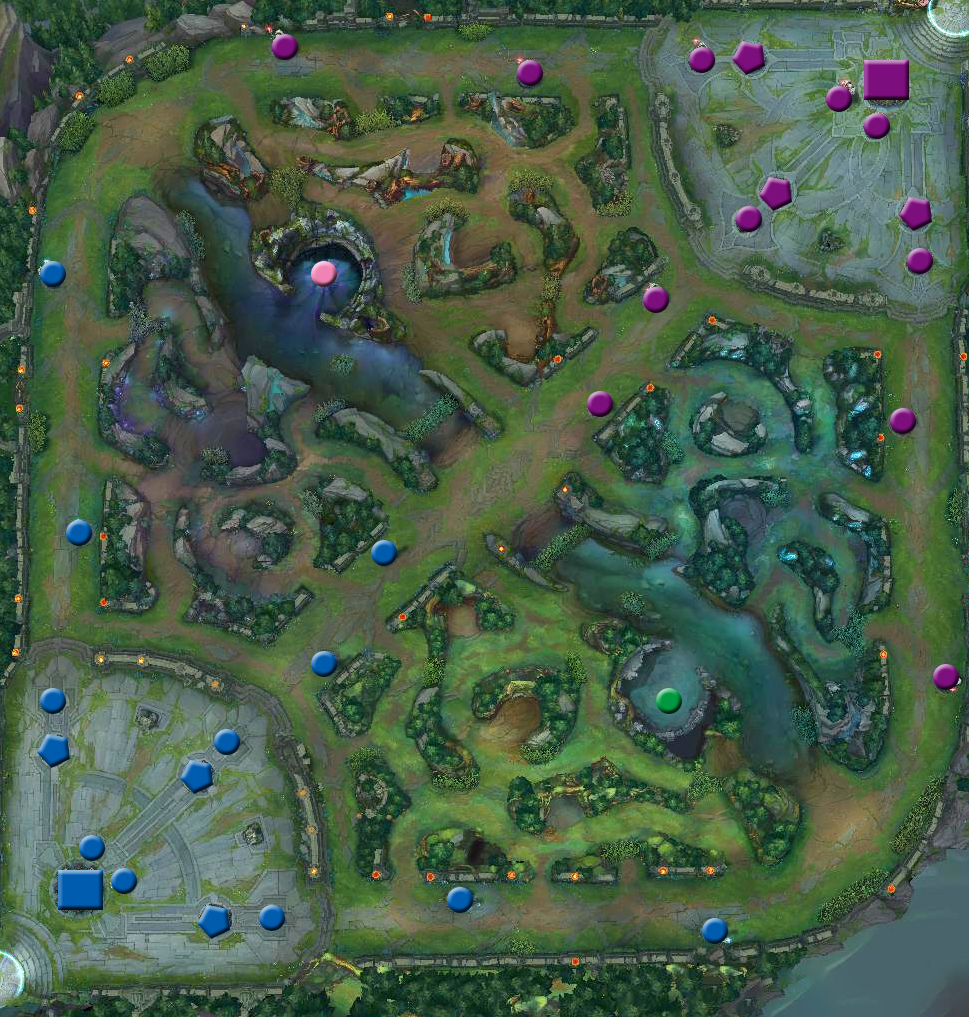
\includegraphics[width=0.5\textwidth]{img/lolmap.jpg}
  \caption{League of Legends map~\cite{lolmap}}\label{fig:lolmap}
\end{figure}

In \Cref{fig:lolmap}, the map is presented, it consists of three lanes identified as \emph{top}, \emph{middle}, and \emph{bottom} which connects the two bases. The blue and purple colours represent the blue and purple teams' respective structures. Circles are \emph{turrets}, pentagons are \emph{inhibitors} and squares are \emph{nexuses}. The green circle indicates \emph{the dragon} and the pink is \emph{the baron}.

\begin{table}[!h]
  \begin{tabular}{l p{13cm}}
    \textbf{Nexus}: & This building spawn \emph{creeps}, which are small monsters with low damage and health, that walks along each of the lanes toward the opposing teams base. Killing these creeps award gold and experience. When the nexus is destroyed the game ends, making the destroying team the winners\\
    \textbf{Inhibitor}: & When this is destroyed, the destroying teams' minions become stronger on the lane where the inhibitor was placed\\
    \textbf{Turret}: & This is a defensive structure, which fires at nearby enemies\\
    \textbf{Jungle}: & The area between the lanes which hosts stronger \emph{monsters}\\
  \end{tabular}
\end{table}

The creeps which are spawned by the nexuses walk toward the opposing teams base, which means they will meet in the middle of the lanes, where the majority of the fighting will take place. Killing the dragon awards the killing team with \emph{dragon slayer}, which is a team wide buff that increases the power of the champions. Killing the baron awards \emph{hand of baron}, which makes the living champions of the killing team, temporarily stronger.

\emph{Experience} and \emph{gold} are the currencies of the game, and they are earned by killing creeps, monsters or opposing champions, both are earned individually by each player. Experience is used to improve the abilities of the champion, while gold is spend purchasing items, that will make the player more powerful.

The game combines strategy, individual player skill, communication, and team play.
With a prize a pool exceeding \$2.000.000 in the 2014 LoL World Championships, the game attracts serious and skilled players~\cite{lolprize}.

%%% Local Variables:
%%% mode: latex
%%% TeX-master: "../main"
%%% End:
